% !TeX spellcheck = id_ID
\documentclass[a4paper,12pt]{article}
\usepackage[indonesian]{babel}
\usepackage{graphicx}
\usepackage{multirow}
\usepackage{enumitem}
\usepackage{listings}
\usepackage{wrapfig}
\usepackage[T1]{fontenc}
\usepackage{inconsolata}
\usepackage{lipsum}
\usepackage{adjustbox}


\usepackage{color}
\usepackage[table]{xcolor}
\definecolor{pblue}{rgb}{0.13,0.13,1}
\definecolor{pgreen}{rgb}{0,0.5,0}
\definecolor{pred}{rgb}{0.9,0,0}
\definecolor{pgrey}{rgb}{0.46,0.45,0.48}
\lstset{language=Java,
	showspaces=false,
	showtabs=false,
	breaklines=true,
	showstringspaces=false,
	breakatwhitespace=true,
	commentstyle=\color{pgreen},
	keywordstyle=\color{pblue},
	stringstyle=\color{pred},
	rulecolor=\color{black},
	basicstyle=\ttfamily,
	moredelim=[il][\textcolor{pgrey}]{$$},
	moredelim=[is][\textcolor{pgrey}]{\%\%}{\%\%}
}

\graphicspath{ {./img/} }
\begin{document}
\title{ {\Large Laporan Praktikum}\\ Algoritma dan Pemrograman \\{\Large Pertemuan 13}}

\author{Aldzikri Dwijayanto Prathama 
	\\195410189
	\\Teknik Informatika}
\makeatletter
\begin{titlepage}
	\begin{center}
		{\huge \bfseries \@title }\\[14ex]
		
\includegraphics[scale=.8]{logo}\\[4ex]
		{\large \@author}\\[19ex]
		{\large \bfseries {SEKOLAH TINGGI MANAJEMEN INFORMATIKA DAN KOMPUTER
				AKAKOM YOGYAKARTA}}
	\end{center}


%{\large \@date} 
\end{titlepage}
\makeatother
%\maketitle
\newpage
\tableofcontents
\newpage

\section{Tujuan}
Mahasiswa dapat menyelesaikan kasus dengan menggabungkan konsep perulangan
dalam seleksi

\section{Dasar Teori}
Seperti yang telah dijelaskan pada modul 12 bahwa Seleksi dan iterasi/perulangan dapat
digabungan dengan dua kemungkinan, yang pertama seleksi dalam perulangan dan yang
kedua adalah perulangan dalam seleksi. Pada modul 13 ini, akan dibahas model yang
kedua yaitu perulangan dalam seleksi. gambaran sederhana dari model ini salah satunya
adalah :

\begin{lstlisting}[frame=single]
    if(kondisi)
    {
        for(ungkapan1;ungkapan2;ungkapan3)
        {
            Statement;
        }
    }
\end{lstlisting}

\section{Praktik}
\subsection{Praktik 1}
\textbf{Program pertama}\\
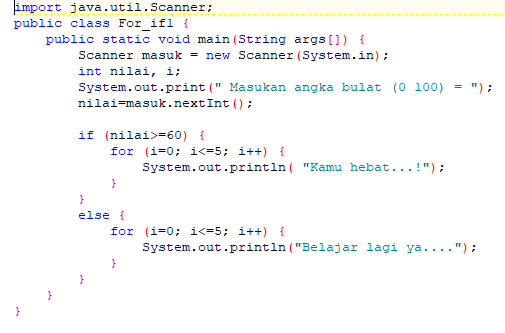
\includegraphics{img1.PNG}\\
Pada program pertama terdapat perulangan for didalam seleksi if.  Pada seleksi if memiliki kondisi nilai $>=$ 60, jadi jika nilai yang dimasukkan oleh user lebih dari sama dengan 60, maka program akan menjalankan perulangan yang pertama yang akan mengeprint kalimat "Kamu hebat...!" sebanyak 6 kali. Sedangkan jika nilai dimasukkan angka lebih kecil dari 60, maka program akan menjalankan perulangan kedua, yang akan mengeprint kalimat "Belajar lagi ya..." sebanyak 6 kali.\\
Jika program dimasukkan bilangan >60 maka outputnya akan seperti berikut:\\
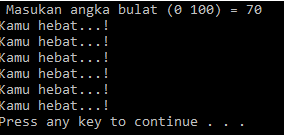
\includegraphics{img2.PNG}\\
\newpage 
Jika program dimasukkan bilangan <60 maka outputnya akan seperti berikut:\\
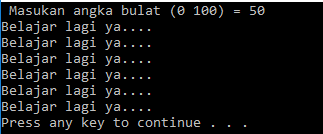
\includegraphics{img3.PNG}\\[4ex]

\textbf{Program Kedua}\\
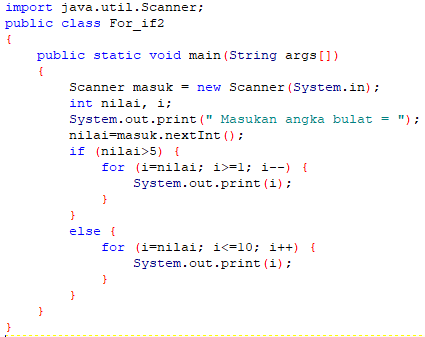
\includegraphics{img4.PNG}\\
Program kedua ini terdapat if yang memiliki kondisi nilai > 5, jadi jika variabel nilai dimasukkan bilangan lebih dari 5, maka program akan melakukan perulangan yang akan mengeprint bilangan yang dimasukkan, lalu dikurangi dengan 1. Perulangan ini akan terus berjalan sampai bilangan tadi tersisa 1. Jadi jika program dijalankan dan diberi nilai > 5 maka outputnya akan seperti berikut:\\
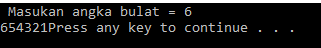
\includegraphics{img5.PNG}\\

Namun jika variabel nilai diberi bilangan kurang dari 5, maka akan masuk ke else, dan program akan melakukan perulangan yang akan mengeprint bilangan yang dimasukkan tadi, lalu ditambah dengan 1 sampai bilangan mencapai 10. Jadi jika program dijalankan dan diberi bilangan < 5 maka outputnya seperti berikut:\\
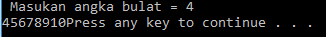
\includegraphics{img6.PNG}

\subsection{Praktik 2}
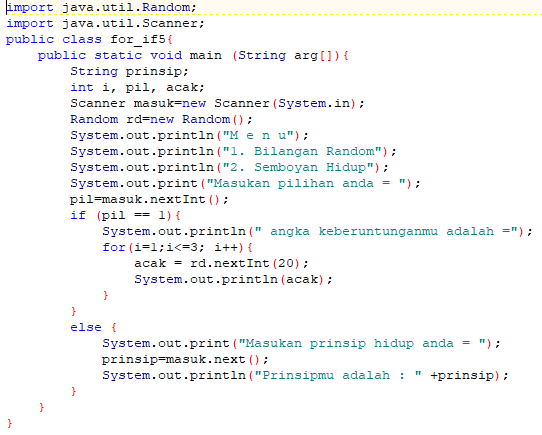
\includegraphics{img7.PNG}\\
Program diatas memiliki seleksi if dengan kondisi pil == 1, jadi jika user memilih opsi 1, maka program akan menjalankan perulangan for yang diulangi sebanyakk 3 kali, yang mana perulangan ini akan mengeprint angka random dari angka 0-19. Output jika user memilih opsi 1 maka akan seperti berikut:\\
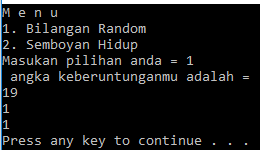
\includegraphics{img8.PNG}\\
Namun jka user memasukkan angka selain 1, maka akan masuk ke else, lalu user disuruh memasukkan prinsip hidupnya, lalu program akan mengeprint kembali kata yang dimasukkan user ke layar. Outputnya seperti berikut:\\
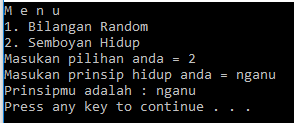
\includegraphics{img9.PNG}

\newpage

\section{Latihan}
Pada sesi latihan, mahasiswa diberi tugas untuk membuat program yang akan menampilkan bilangan ganjil atau genap yang nanti akan dipilih oleh user, yang panjang bilangannya juga ditentukan oleh user.\\
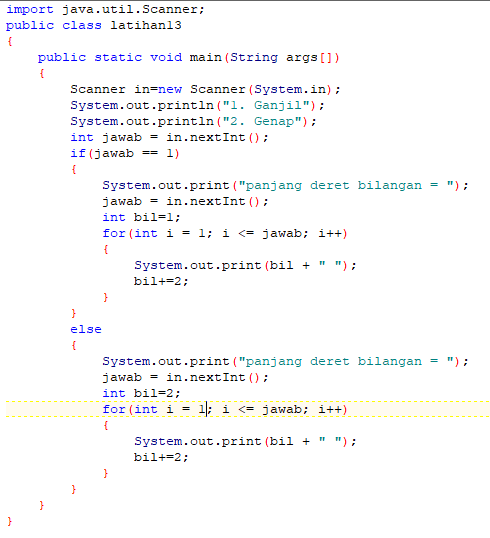
\includegraphics{img10.PNG}\\
Program diatas memiliki seleksi dengan kondisi jawab == 1, jadi jika user memilih opsi 1, maka program akan menjalankan perulangan for yang akan menampilkan variabel bil, setelah itu menambahkannya dengan 2, perulangan akan terus berjalan sampai nilai variabel i sama dengan nilai di variabel jawab. Sehingga perulangan ini akan menampilan bilangan ganjil yang jumlah deretnya sebanyak yang diinginkan oleh user. Output jika user memilih bilangan ganjil adalah sebagai berikut:\\
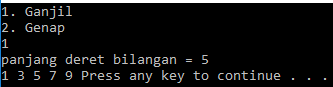
\includegraphics{img11.PNG}\\
Jika user memilih opsi selain 1, maka program akan menjalankan perulangan sama seperti di dalam if, yang berbeda adalah variabel bil diberi niali awal 2, sehingga perulangan ini menghasilkan deret bilangan genap. Outputnya seperti berikut:\\
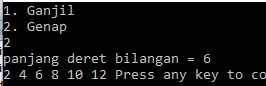
\includegraphics{img12.PNG}

\newpage

\section{Tugas}
Pada tugas, mahasiswa membuat program dalam suatu menu untuk menghitung bilangan Fibonacci dan Faktorial\\
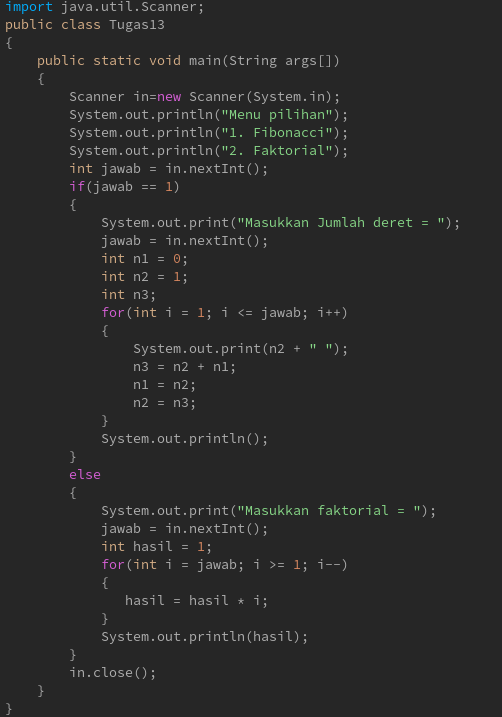
\includegraphics[width=0.8\linewidth]{tugas1.png}\\
Jika user memasukkan bilangan 1, maka program akan menjalankan perulangan untuk fibonacci. Untuk membuat operasi fibonacci variabel n1, n2, dan n3 diinisialisasi sebagai integer, dengan n1 diberi nilai 0, dan n2 diberi nilai 1. Pada perulangan for, program akan mengeprint nilai dari n2, setelah itu n3 diberi nilai dari hasil penjumlahan n2, dan n1. Lalu n1 nilainya diganti dengan nilai n2, dan n2 nilainya diganti dengan nilai n3. Perulangan akan terus berjalan sampai batas yang
ditentukan oleh user. Output untuk perulangan fibonacci adalah sebagai berikut:\\
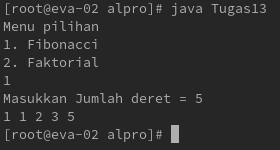
\includegraphics[scale=.8]{tugas2.png}\\
Sedangkan jika dimasukkan selain 1,  maka program akan melakukan perulangan untuk faktorial. Di dalam perulangan for, variabel hasil akan diganti nilainya dari hasil operasi perkalian variabel hasil dan variabel i. Maka outputnya seperti berikut:\\
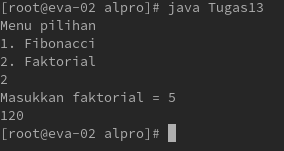
\includegraphics[scale=.8]{tugas3.png}

\newpage

\section{Kesimpulan}
Setelah praktik ini mahasiswa dapat menyelesaikan kasus dengan menggabungkan konsep perulangan dalam seleksi

\end{document}
